% latex table generated in R 3.2.2 by xtable 1.8-0 package
% Wed Jan 27 11:17:04 2016
{\setlength{\tabcolsep}{0.3em}}
{\renewcommand{\arraystretch}{1}}% for the vertical padding
% \small
\begin{tabular}{%
  l>{\centering\arraybackslash}%
  m{1.5cm}>{\centering\arraybackslash}%
  m{3.0cm}>{\centering\arraybackslash}%
  m{1.7cm}cccc>{\centering\arraybackslash}%
  m{2.7cm}>{\centering\arraybackslash}%
  m{2.7cm}>{\centering\arraybackslash}%
  m{1.1cm}cc%
}%
\toprule
  & \multirow[c]{2}*{\textbf{Problem}}
  & \multicolumn{6}{c}{\textbf{Network Properties}}
  & \multicolumn{2}{c}{\textbf{Complexity} }
  & \multicolumn{3}{c}{\textbf{Algorithms}}
  \\
%-------------------------------------------------------------------------------
%-------------------------------------------------------------------------------
 \cmidrule(lr){3-8}\cmidrule(lr){9-10}\cmidrule(lr){11-13}
  &
  & \multicolumn{1}{c}{Graph Structure}
  & \multicolumn{1}{c}{Example}
  & \screentextcolor{GENERATOR}{$\fmagnitude{\generators}$} 
  & \screentextcolor{CONSUMER}{$\fmagnitude{\consumers}$}
  & \screentextcolor{SUSCEPTANCE}{$\susceptance$}
  & \screentextcolor{CAPACITY}{$\capacity$}
  & \multicolumn{1}{c}{Hardness}
  & \multicolumn{1}{c}{Reference}
  & \multicolumn{1}{c}{Name} 
  & \multicolumn{1}{c}{\screentextcolor{SUSCEPTANCE}{$\susceptance$}}
  & \multicolumn{1}{c}{\screentextcolor{CAPACITY}{$\capacity$}}
  \\
%-------------------------------------------------------------------------------
%-------------------------------------------------------------------------------
 \midrule\addlinespace
%-------------------------------------------------------------------------------
%-------------------------------------------------------------------------------
\rowcolor{Table-Line-Marker}
%-------------------------------------------------------------------------------
1\label{ch:facts:sec:exploit_structural_characteristics:tbl:tree}
& \acrshort{mffp} and~\acrshort{offp}
& tree graphs
& \raisebox{-0.5cm}[0pt][0pt]{
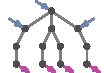
\includegraphics{switchplacement/figures/graph_structure-tree.pdf}%
}
& \screentextcolor{GENERATOR}{$\infty$}
& \screentextcolor{CONSUMER}{$\infty$}
& \screentextcolor{SUSCEPTANCE}{--}
& \screentextcolor{CAPACITY}{--}
& polynomial-time solvable
& \cref{ch:network-analyzes:sec:mathematical-model:lem:pf-matrix-is-tum},
\cref{ch:facts:thm:fvs}, 
\cref{ch:foundations:sec:graph-theoretical-flows} p.\
\pageref{ch:foundations:sec:graph-theoretical-flows:para:maximum-flow-problem}
& \acrshort{mf}
& \screentextcolor{SUSCEPTANCE}{$\infty$}
& \screentextcolor{CAPACITY}{$\infty$}
\\\addlinespace\addlinespace
% 
2\label{ch:switching:sec:exploit_structural_characteristics:tbl:series_parallel}
& \acrshort{mffp} and~\acrshort{offp}
& series-parallel graphs
& 
\raisebox{-0.5cm}[0pt][0pt]{%
  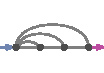
\includegraphics{switchplacement/figures/graph_structure-series_parallel_graph.pdf}%
}%
& \screentextcolor{GENERATOR}{$\infty$}
& \screentextcolor{CONSUMER}{$\infty$}
& \screentextcolor{SUSCEPTANCE}{$\infty$}
& \screentextcolor{CAPACITY}{$\infty$}
& --%\NP-hard
& --%\parencite[pp. 10; Theorem 4]{Leh15a}
& --
& \screentextcolor{SUSCEPTANCE}{--}
& \screentextcolor{CAPACITY}{--}
\\\addlinespace\addlinespace
% 
\rowcolor{Table-Line-Marker}
%-------------------------------------------------------------------------------
3\label{ch:facts:sec:exploit_structural_characteristics:tbl:cactus}
& \acrshort{mffp} and~\acrshort{offp}
& cacti with maximum degree of~$3$
& \raisebox{-0.5cm}[0pt][0pt]{%{-\totalheight}
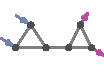
\includegraphics{switchplacement/figures/graph_structure-cacti_graph.pdf}}
& \screentextcolor{GENERATOR}{$\infty$}
& \screentextcolor{CONSUMER}{$\infty$}
& \screentextcolor{SUSCEPTANCE}{$\infty$}
& \screentextcolor{CAPACITY}{$\infty$}
& \NP-hard
& \parencite[pp.10; Theorem 4]{Leh15a}
& --
& \screentextcolor{SUSCEPTANCE}{--}
& \screentextcolor{CAPACITY}{--}
\\\addlinespace\addlinespace
% 
4\label{ch:switching:sec:exploit_structural_characteristics:tbl:plane_graph}
& \acrshort{mffp} and~\acrshort{offp}
& planar graph with~$\max$ degree of~$3$
& \raisebox{-0.5cm}[0pt][0pt]{%
  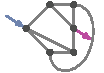
\includegraphics{switchplacement/figures/graph_structure-plane_graph.pdf}
}%
& \screentextcolor{GENERATOR}{$\infty$}
& \screentextcolor{CONSUMER}{$\infty$}
& \screentextcolor{SUSCEPTANCE}{$\infty$}
& \screentextcolor{CAPACITY}{$\infty$}
& --
& --
& --
& \screentextcolor{SUSCEPTANCE}{--}
& \screentextcolor{CAPACITY}{--}
\\\addlinespace\addlinespace
% 
\rowcolor{Table-Line-Marker}
%-------------------------------------------------------------------------------
5
\label{ch:facts:sec:exploit_structural_characteristics:tbl:arbitrary_graph}
& \acrshort{mffp} and~\acrshort{offp}
& arbitrary graphs
& \raisebox{-0.5cm}[0pt][0pt]{%{-\totalheight}

\includegraphics{switchplacement/figures/graph_structure-arbitrary_graph.pdf}%
}%
& \screentextcolor{GENERATOR}{$\infty$}
& \screentextcolor{CONSUMER}{$\infty$}
& \screentextcolor{SUSCEPTANCE}{$\infty$}
& \screentextcolor{CAPACITY}{$\infty$}
& strongly~\NP-hard
& \parencite[pp.7; Theorem 1]{Leh15a}
& --
& \screentextcolor{SUSCEPTANCE}{--}
& \screentextcolor{CAPACITY}{--}
\\\addlinespace\addlinespace
% 
%-------------------------------------------------------------------------------
%-------------------------------------------------------------------------------
   \bottomrule
\end{tabular}
